\documentclass[aspectratio=169,12pt]{beamer}
\usetheme{Madrid}
\usecolortheme{dolphin}
\usefonttheme{professionalfonts}
\setbeamertemplate{navigation symbols}{}
\setbeamertemplate{footline}{}

\usepackage[T1]{fontenc}
\usepackage[utf8]{inputenc}
\usepackage{graphicx}
\usepackage{amsmath,amssymb}
\usepackage{hyperref}
\usepackage{siunitx}
\usepackage{physics}
\usepackage{tikz}

\begin{document}

\title[Chapter 2]{Chapitre 2: Vecteurs, qubit et superposition}
\author{JAMOTTE Maxime, SCHOONEN Cédric}
\institute{Digital Learning Hub}
\date{}

\begin{frame}
  \titlepage
\end{frame}

\begin{frame}{Objectifs du chapitre 2}
  \begin{enumerate}
    \item Vecteurs\\~\\
    %\item Produit scalaire\\~\\
    \item Qubit, superposition d'états et vecteurs\\~\\
    \item Mesure de l'état d'un qubit
  \end{enumerate}
\end{frame}

\begin{frame}{Vecteurs}
  {%
    \setbeamercolor{itemize/enumerate body}{fg=gray!60}
    \setbeamercolor{itemize item}{fg=gray!60}
    \setbeamercolor{alerted text}{fg=black}
    \begin{columns}[T]
      \begin{column}{0.55\textwidth}
        \begin{itemize}[<+-| alert@+>]
          \setlength{\itemsep}{0.6em}
          \item Définition d'un vecteur
          \item Addition de vecteurs
          \item Multiplication d'un vecteur par une constante
        \end{itemize}
        \bigskip
        \only<1>{\[
          \vec r = \begin{pmatrix} a \\ b \end{pmatrix}
        \]}
        \only<2>{\[
          \vec r + \vec p = 
          \begin{pmatrix} a \\ b \end{pmatrix} +
          \begin{pmatrix} c \\ d \end{pmatrix} =
          \begin{pmatrix} a+c \\ b+d \end{pmatrix}
        \]}
        \only<3>{\[
          \lambda \begin{pmatrix} a \\ b \end{pmatrix} =
          \begin{pmatrix} \lambda a \\ \lambda b \end{pmatrix}
        \]}
      \end{column}
      \begin{column}{0.4\textwidth}
        \centering
        \only<1>{
\includegraphics[width=\linewidth]{figures/vecteur.png}}
        \only<2>{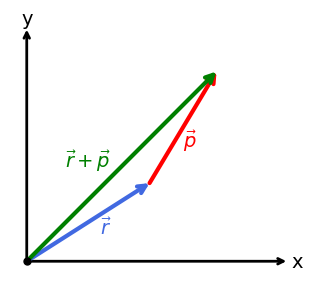
\includegraphics[width=\linewidth]{figures/add_vecteurs.png}}
        \only<3->{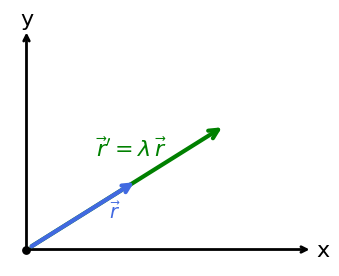
\includegraphics[width=\linewidth]{figures/multiplication_nombre.png}}
      \end{column}
    \end{columns}
  }
\end{frame}

\begin{frame}{Qubit}
  \begin{itemize}[<+->]
    \setlength{\itemsep}{0.6em}
    %\item Electron autour du noyau: infinité de positions possibles.
    \item L'électron passe à travers les fentes du haut ($H$) et du bas ($B$) en même temps.% $\ket{\psi_e^{}} = \alpha \ket{H} + \beta \ket{B}$.
      \only<1->{%
        \vspace{0.5em}
        \begin{center}
          \begin{minipage}{0.42\textwidth}
            \centering
            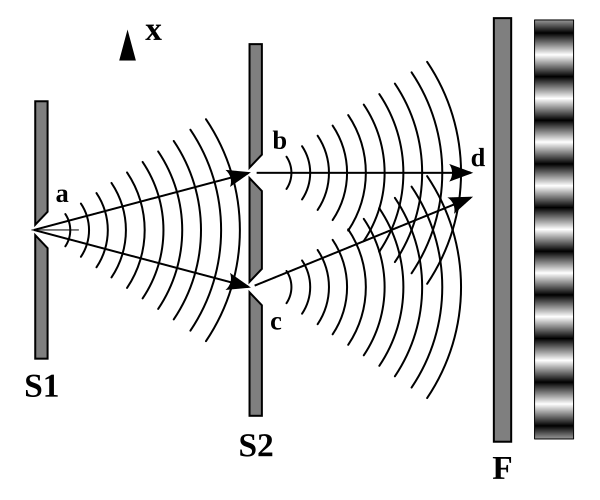
\includegraphics[width=0.6\linewidth]{figures/fente_Young.png}
          \end{minipage}\hfill
          \begin{minipage}{0.42\textwidth}
            \centering
            \only<2->{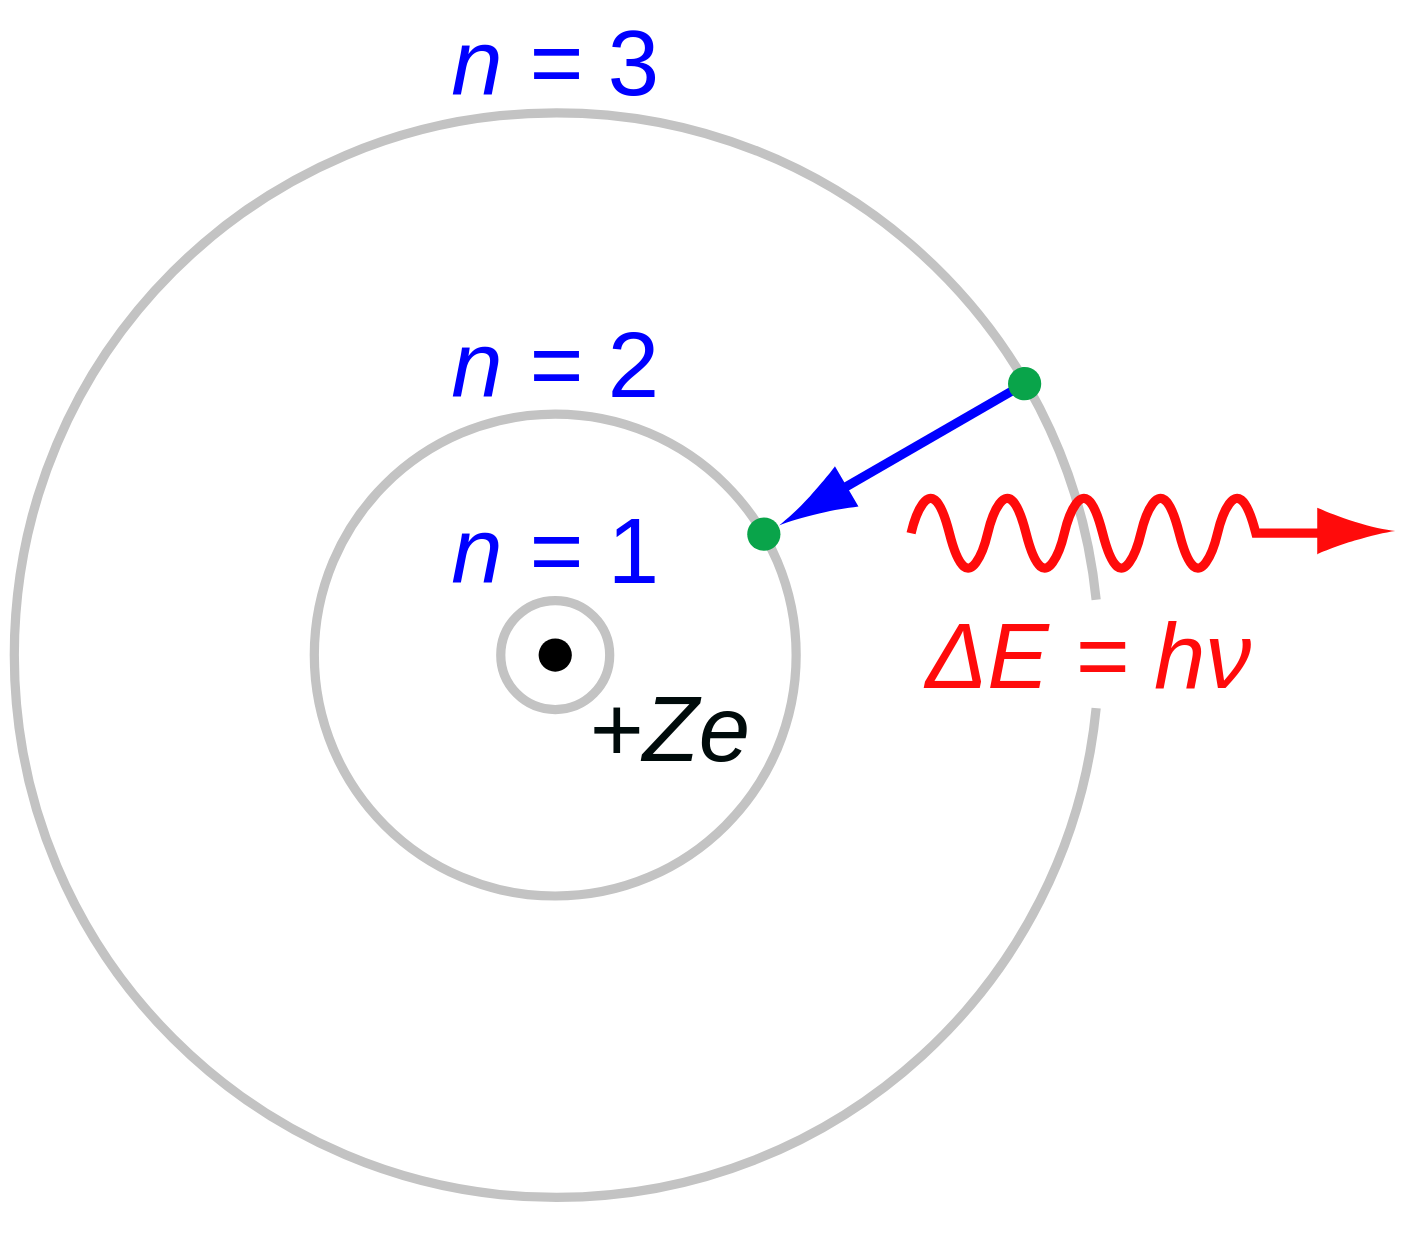
\includegraphics[width=0.6\linewidth]{figures/bohr_model.png}}
          \end{minipage}
        \end{center}
      }
    \item Certains systèmes physiques ont des niveaux discrets d'énergie (au lieu de la position).
    \item \textbf{Qubit} (= bit quantique) = système quantique à 2 niveaux, notés $\ket 0$ et $\ket 1$.
  \end{itemize}
\end{frame}

\begin{frame}{Superposition d'états et vecteurs}
  \begin{columns}[T]
    \begin{column}{0.65\textwidth}
      \begin{itemize}[<+->]
        \item Un qubit peut être dans $\ket 0$, $\ket 1$ ou toute \textbf{superposition} des deux: $\alpha \ket 0 + \beta \ket 1$.
        \item Superposition = combinaison linéaire d'états.
        % \item \textbf{Postulat} : les états quantiques forment un espace vectoriel (espace de Hilbert). Une combinaison linéaire d'états est aussi un état.
        \item L'état superposé $\ket {\psi} = \alpha \ket 0 + \beta \ket 1$, s'écrit $\begin{pmatrix} \alpha \\ \beta \end{pmatrix}$,\\~\\
        \item Chaque \textbf{qubit} est identifiable à la \textbf{direction} de son vecteur.
        \item $\ket{0}$ et $-\ket{0}$ correspondent au même état quantique.
        %\item Probabilités de mesure : $P(\ket 0)=|\alpha|^2$, $P(\ket 1)=|\beta|^2$,
        %$$ \Longrightarrow  |\alpha|^2 + |\beta|^2 = 1$$
      \end{itemize}
    \end{column}
    \begin{column}{0.35\textwidth}
      \vspace{2em}
      \centering
      $\ket 0 = \begin{pmatrix}1 \\ 0\end{pmatrix}$ et $\ket 1 = \begin{pmatrix}0 \\ 1\end{pmatrix}$\\~\\~\\
      \only<4->{\resizebox{0.8\textwidth}{!}{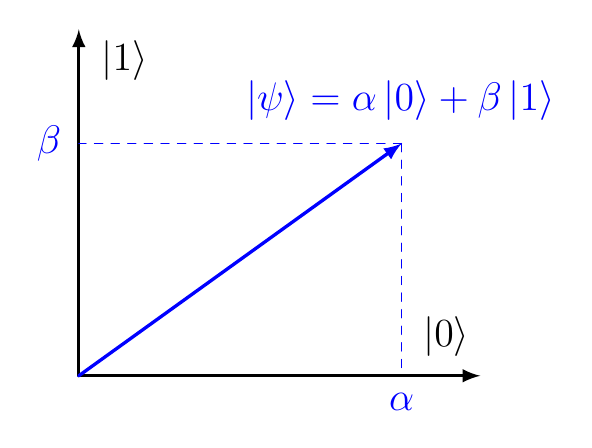
\begin{tikzpicture}[x=1cm,y=1cm,line cap=round,line join=round,>=latex]
  % Axes
  \draw[black,very thick,->] (0,0) -- (0,4.4);
  \draw[black,very thick,->] (0,0) -- (5.1,0);

  % State vector
  \draw[blue,very thick,->] (0,0) -- (4.1,2.95);
  \draw[blue,dashed] (4.1,2.95) -- (4.1,0);
  \draw[blue,dashed] (4.1,2.95) -- (0,2.95);

  % Labels
  \node[anchor=west,font=\Large] at (2.0,3.5) {\textcolor{blue}{$\ket{\psi} = \alpha \ket{0} + \beta \ket{1}$}};
  \node[anchor=north,text=blue,font=\Large] at (4.1,-0.1) {$\alpha$};
  \node[anchor=east,text=blue,font=\Large] at (-0.1,2.95) {$\beta$};

  \node[anchor=east,font=\Large] at (1.0,4.0) {$\ket{1}$};
  \node[anchor=west,font=\Large] at (4.25,0.5) {$\ket{0}$};
\end{tikzpicture}
}}
    \end{column}
  \end{columns}
\end{frame}


\begin{frame}{Mesure de l'état d'un qubit}
  \begin{columns}[T]
    \begin{column}{0.65\textwidth}
      \begin{itemize}[<+->]
      \item Mesurer = extraire de l'information\\~\\
      \item L'interaction avec l'appareil de mesure détruit la superposition\\~\\
      \item Etat final est alors soit $\ket 0$, soit $\ket 1$.\\~\\
      \item Probabilité de mesurer l'état $\ket 0$: $P(\ket 0)=|\alpha|^2$\\
      Probabilité de mesuer l'état $\ket 1$: $P(\ket 1)=|\beta|^2$\\~\\
      \item C'est l'origine de l'équivalence entre $\ket 0$ et $-\ket 0$.
\end{itemize}
    \end{column}
    \begin{column}{0.35\textwidth}
      \vspace{2em}
      \centering
      $\ket 0 = \begin{pmatrix}1 \\ 0\end{pmatrix}$ et $\ket 1 = \begin{pmatrix}0 \\ 1\end{pmatrix}$\\~\\~\\
      \only<4->{\resizebox{0.8\textwidth}{!}{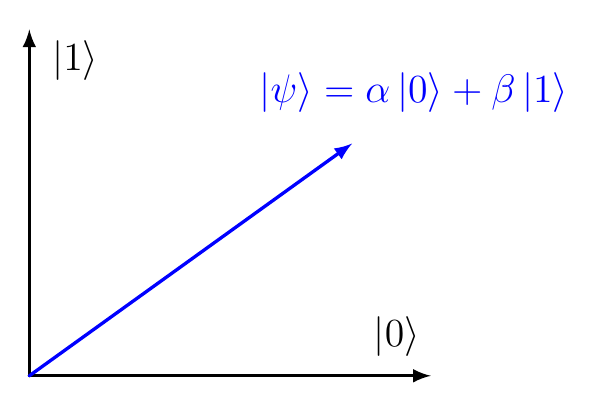
\begin{tikzpicture}[x=1cm,y=1cm,line cap=round,line join=round,>=latex]
  % Axes
  \draw[black,very thick,->] (0,0) -- (0,4.4);
  \draw[black,very thick,->] (0,0) -- (5.1,0);

  % State vector
  \draw[blue,very thick,->] (0,0) -- (4.1,2.95);

  % Labels
  \node[anchor=west,font=\Large] at (2.8,3.6) {\textcolor{blue}{$\ket{\psi} = \alpha \ket{0} + \beta \ket{1}$}};

  \node[anchor=east,font=\Large] at (1.0,4.0) {$\ket{1}$};
  \node[anchor=west,font=\Large] at (4.25,0.5) {$\ket{0}$};
\end{tikzpicture}
}}
    \end{column}
  \end{columns}
\end{frame}

\begin{frame}{Probabilité et produit scalaire}
      \begin{itemize}[<+->]
        \setlength{\itemsep}{0.6em}
        \item Produit scalaire entre deux états quantiques: $\braket{\phi}{\psi}$\\~\\
        \item Il se traduit par un produit scalaire entre leurs vecteurs associés:\\
         $$\ket \psi = \begin{pmatrix} \alpha \\ \beta \end{pmatrix},\quad  \ket \phi = \begin{pmatrix} \gamma \\ \delta \end{pmatrix} \qquad \braket{\phi}{\psi} =  \gamma^*\alpha + \delta^*\beta$$\\~\\
        \item Exemples: $\qquad \braket{0}{0} = 1, \qquad \braket{0}{1} = 0, \qquad \braket{1}{1} = 1$\\~\\
        \item La probabilité d'obtenir un résultat de mesure $\ket  0$ ou $\ket 1$ se calcule à partir du produit scalaire entre $\ket \psi$ et $\ket 0$ ou $\ket 1$:
        $$ |\braket{0}{\psi}|^2 = |\alpha|^2, \qquad  |\braket{1}{\psi}|^2 = |\beta|^2$$
      \end{itemize}
\end{frame}


\begin{frame}{Fin du chapitre 2}
  \begin{enumerate}
    \item Vecteurs\\~\\
    %\item Produit scalaire\\~\\
    \item Qubit, superposition d'états et vecteurs\\~\\
    \item Mesure de l'état d'un qubit
  \end{enumerate}
\end{frame}

\end{document}
